\documentclass[]{fithesis3}
\usepackage[
	main=czech,
	english
]{babel}

\thesissetup{
    date          = \the\year/\the\month/\the\day,
    university    = mu,
    faculty       = fi,
    type          = bc,
    author        = Ondřej Přikryl,
    gender        = m,
    advisor       = {RNDr. Michal Procházka, Ph.D.},
    title         = {Integrace RemSig do klientských aplikací},
    keywords      = {remsig, pkcs11, csp, oauth2.0, ...},
}

\begin{document}
\chapter{Úvod}

Prvky informačních technologií se stávají každodenní součástí života a většina lidí by si bez nich již nedokázala život představit. Informační technologie uživatelům v mnoha směrech usnadňují život. Slouží jak k práci, tak i ke komunikaci se známými, zábavě a mnoha dalším činnostem. S rozšířením se však zvyšuje i potenciální riziko, které zneužití těchto prvků přináší. V době, kdy internet poskytuje základní komunikaci mezi více než miliardou lidí a je čím dál tím více používán jako nástroj k obchodování, se bezpečnost stává nesmírně důležitou otázkou, která by neměla zůstat nepovšimnuta. Částečnou odpovědí na tuto otázku bylo zavedení kryptografických systémů. I ty však nenabízí řešení ve všech případech a lidé by si měli stále dávat velký pozor. Kryptografie nebyla původní součástí návrhu internetu, ale v posledních dekádách se díky rozmachu digitálních technologií stala důležitým prvkem internetové infrastruktury. Přestože je skryta před zraky laických uživatelů, jde o důležitý vědní obor, který v současnosti prožívá obrovský posun kupředu. Tento vývoj je způsoben zejména tím, že si uživatelé začínají uvědomovat potřebu chránit své data a soukromí i ve virtuálním světě. Moderní kryptografie má mnoho podob a odvětví, jednou z nich je digitální podpis (též nazýván elektronický podpis), který je nezbytnou součástí systému RemSig.

Digitální podpis slouží k nahrazení obyčejného podpisu v digitálním světě. Tento podpis je jednoznačně spojen s uživatelskou entitou (autentizace), kterou může být jak běžný domácí uživatel, tak i organizace nebo státní útvar (digitální značka). Majitel digitálního podpisu je vždy dohledatelný. Společně s autentizací zajišťuje také integritu. Integrita zaručuje, že data nebyla po cestě pozměněna. To je velice důležité k ujištění, že data, která byla odeslána, druhá strana také přijala. To bez digitálního podpisu není tak samozřejmé, jak by se mohlo zdát. Digitální podpis je tvořen tzv. certifikátem, který je vydáván certifikační autoritou.

Systém RemSig je bezpečné vzdálené úložiště certifikátů a privátních klíčů, které uživatelům poskytuje možnost podepisovat dokumenty bez nutnosti neustálého fyzického přístupu k zařízení, na němž je certifikát uložen. Díky tomu odpadá uživatelům systému RemSig povinnost nosit s sebou hardwarové zařízení, což zvyšuje uživatelskou přívětivost i funkcionalitu. Uživatelé totiž mohou podepisovat dokumenty, i když u sebe právě nemají token1, nebo když jsou na jiném počítači, který není nakonfigurovaný pro práci s digitálními podpisy nebo není důvěryhodný.

RemSig umožňuje podepisování dokumentů přímo z webového rozhraní systému INET a IS MU a je v souladu se současnou českou legislativou. RemSig je napojen na služby certifikační autority PostSignum2, což je další výhodou pro zaměstnance MU, kteří tak nemusí řešit vydání certifikátu třetí stranou, ale vše si nastaví v rozhraní INET.

Důležitou součástí RemSig je uživatelská přívětivost, a proto je nutná implementace funkcí do dalších operačních systémů. V současné době systém plně nespolupracuje s operačním systémem Windows a je pro něj potřeba tyto funkce implementovat, což je náplní mé bakalářské práce. V jejím rámci implementuji rozhraní pro práci s certifikáty v systému Windows, které bude kompatibilní s požadavky systému RemSig. V první fázi práce se zaměřuji na vytvoření knihovny v programovacím jazyce C. Tato knihovna obsahuje základní funkce pro práci s úložištěm certifikátů v operačním systému Windows pomocí vývojového prostředí Cryptography API: Next Generation3 (dále CNG). V druhé fázi je zapotřebí vytvořit knihovnu poskytující komunikaci mezi klientem a serverem a pomocí otevřeného protokolu OAuth2 získat přístup k datům uloženým na serveru RemSig. V poslední fázi spojuji již implementované knihovny do fungujícího celku.

Výsledkem mé bakalářské práce je knihovna propojující RemSig a operační systém Windows. Důsledkem toho již není zapotřebí používat webové rozhraní INET a IS MU, což zaměstnancům MU výrazně usnadní práci při podepisování digitálních dokumentů. Nezávislost systému na webovém rozhraní univerzity také umožňuje jeho rozšíření mimo univerzitní kruhy. Dalším krokem při vývoji systému RemSig by mohla být integrace jeho funkcí do systémů iOS a Linux. Podpora těchto tří operačních systémů by RemSigu umožnila fungovat na většině desktopových počítačů na světě.

\chapter{Motivace}

Text text text

\chapter{RemSig}

Systém RemSig je bezpečné vzdálené úložiště certifikátů a privátních klíčů, které uživatelům poskytuje možnost podepisovat dokumenty bez nutnosti neustálého fyzického přístupu k zařízení, na němž je certifikát uložen. Díky tomu odpadá uživatelům systému RemSig povinnost nosit s sebou hardwarové zařízení, což zvyšuje uživatelskou přívětivost i funkcionalitu. Uživatelé totiž mohou podepisovat dokumenty, i když u sebe právě nemají token1, nebo když jsou na jiném počítači, který není nakonfigurovaný pro práci s digitálními podpisy nebo není důvěryhodný.

RemSig umožňuje podepisování dokumentů přímo z webového rozhraní systému INET a IS MU a je v souladu se současnou českou legislativou. RemSig je napojen na služby certifikační autority PostSignum2, což je další výhodou pro zaměstnance MU, kteří tak nemusí řešit vydání certifikátu třetí stranou, ale vše si nastaví v rozhraní INET.

\chapter{OAuth 2.0}

OAuth 2.0 (RFC 6749) je autorizační protokol (resp. framework), který umožňuje aplikacím třetích stran získat přístup ke službám HTTP (k webovým službám?), a to buď jménem registrovaného uživatele anebo ve jménu aplikace třetí strany. Protokol specifikuje pouze autentizaci klienta a výdej přístupového tokenu, přístup k jednotlivým zdrojům je již zcela nezávislý na protokolu. Je tedy zapotřebí nějaké API serveru. Protokol OAuth 2.0 nahrazuje starý protokol OAuth 1.0 a není s ním zpětně kompatibilní.

	\section{Motivace}

	V tradičním modelu autentizace klient-server, žádá-li uživatel o přístup k zabezpečenému 			obsahu, je zapotřebí jeho autentizace pomocí přihlašovacích údajů. Aby tedy aplikace třetí 			strany mohla přistoupit k témuž obsahu, je zapotřebí s ní sdílet přihlašovací údaje oprávněné 		osoby. To však s sebou přináší několik problémů:

		\begin{itemize}
  		\item 
		Aplikace třetích stran si uchovávají přihlašovací údaje k budoucímu použití. Údaje bývají 			většinou uchovávány v otevřené podobě. Uchovávání pouze otisku je nedostatečné.

 		 \item 
		Uživatel ve většině případech nemůže omezit přístup aplikace k chráněnému obsahu, a to 			jak časovou platností, tak i omezením obsahu, ke kterému získá aplikace přístup.

 		 \item 
		Ve většině případech lze odebrat přístup aplikaci ke zabezpečenému obsahu pouze 				změnou hesla. To se však projeví i u dalších aplikací, které jsou závislé na stejných 				přihlašovacích údajích.

  		\item 
		Kompromitace aplikace třetí strany znamená kompromitaci přihlašovacích údajů 					uživatele a všech souborů na nich závislých.
		\end{itemize}

	OAuth tyto problémy řeší zavedením autorizační vrstvy a oddělením rolí klienta 					(aplikace) a vlastníka chráněného zdroje. V protokolu aplikace zažádá o přístup ke 				chráněnému obsahu  a jsou ji přiděleny přihlašovací údaje (přístupový token) odlišné od 			přihlašovacích údajů uživatele. 

	\section{Role}
		OAuth 2.0 definuje 4 typy rolí:

		\begin{itemize}
 		\item Vlastník zdrojů:
  		\newline
		Entita schopná přidělit přístup ke chráněnému obsahu. Jedná-li se o osobu, nazýváme ji 			koncový uživatel.
  		\item Server zdrojů:
  		\newline
		Poskytovatel a hostitel chráněného zdroje, schopný obsluhovat požadavky ke 					chráněnému zdroji pomocí přístupového tokenu.
 	 	\item Klient:
  		\newline
		Aplikace, která vyžaduje přístup ke chráněnému obsahu.
  		\item Server zdrojů:
 		\newline
		Server, který vydává klientovi přístupový token po úspěšné autentizaci oprávněné osoby.
		\end{itemize}
		Protokol nijak nespecifikuje interakci mezi autorizačním serverem a serverem zdrojů. 				Může se jednat o nezávislé entity, ale i o jeden server.

	\section{Přístupový token}	

	Pokaždé když klient potřebuje přistoupit k chráněnému obsahu, potřebuje přístupový token 			(anglicky access token). Přístupový token je řetězec znaků, který oprávňuje klienta k přístupu 		k chráněnému obsahu. V řetězci jsou skrytě uloženy informace o délce platnosti tokenu, o 			rozsahu přístupu k 	chráněnému obsahu a informace o vlastníkovi obsahu.

	\section{Obnovující token}	

	Obnovující token (anglicky refresh token) je získán společně s přístupovým tokenem a slouží k 		obnovení přístupového tokenu po vypršení jeho platnosti. Možnost získání přístupového 			tokenu pomocí obnovujícího tokenu bývá ve většině případech omezena počtem. 

	\section{Průběh protokolu}

	OAuth definuje několik základních způsobů autorizace vedoucích k získání přístupového 			tokenu. Patří mezi ně:

		\begin{itemize}
 		\item Autorizačním kódem:
  		\newline
		Jedná se o doporučený průběh, ke kterému je zapotřebí uživatelský agent 						(prohlížeč). Klient s použitím prohlížeče přesměruje uživatele na přihlašovací stránku. Po 			úspěšné autentizaci zašle autorizační server klientovi autorizační kód. Klient pro získání 			přístupového tokenu zašle autorizační kód autorizačnímu serveru.
  		\item Implicitně:
  		\newline
		Tento typ je zjednodušením průběhu autorizačním kódem. Slouží pro aplikace běžící 				v prohlížeči, které používají skriptovací jazyky jako je například JavaScript. Narozdíl od 			předchozího typu, klient získá přístupový token přímo po přihlášení. Tento typ je rychlejší, 			jelikož redukuje počet výzev a odpovědí, které je potřeba udělat pro získání tokenu.
 	 	\item Zasláním přihlašovacích údajů:
  		\newline
		V tomto typu uživatel poskytne přihlašovací údaje klientovi. Klient zašle přihlašovací údaje 		autorizačnímu serveru, který po úspěšné autentizaci uživatele zašle zpět přístupový 				token. Přihlašovací údaje jsou použity jen pro získání přístupového a obnovujícího tokenu, 			není tedy potřeba jejich uložení pro budoucí použití. Tento typ je používán pouze při 				vysoké důvěře mezi uživatelem a aplikací. 
		\end{itemize}
		
	\newpage
	\section{Praktická část}

	V praktické části jsem implementoval funkce standartního způsobu autorizace autorizačním 			kódem. Parametry jsou zasílané ve formě POST.

	\begin{figure}
  		\begin{minipage}{1.00\textwidth}
    			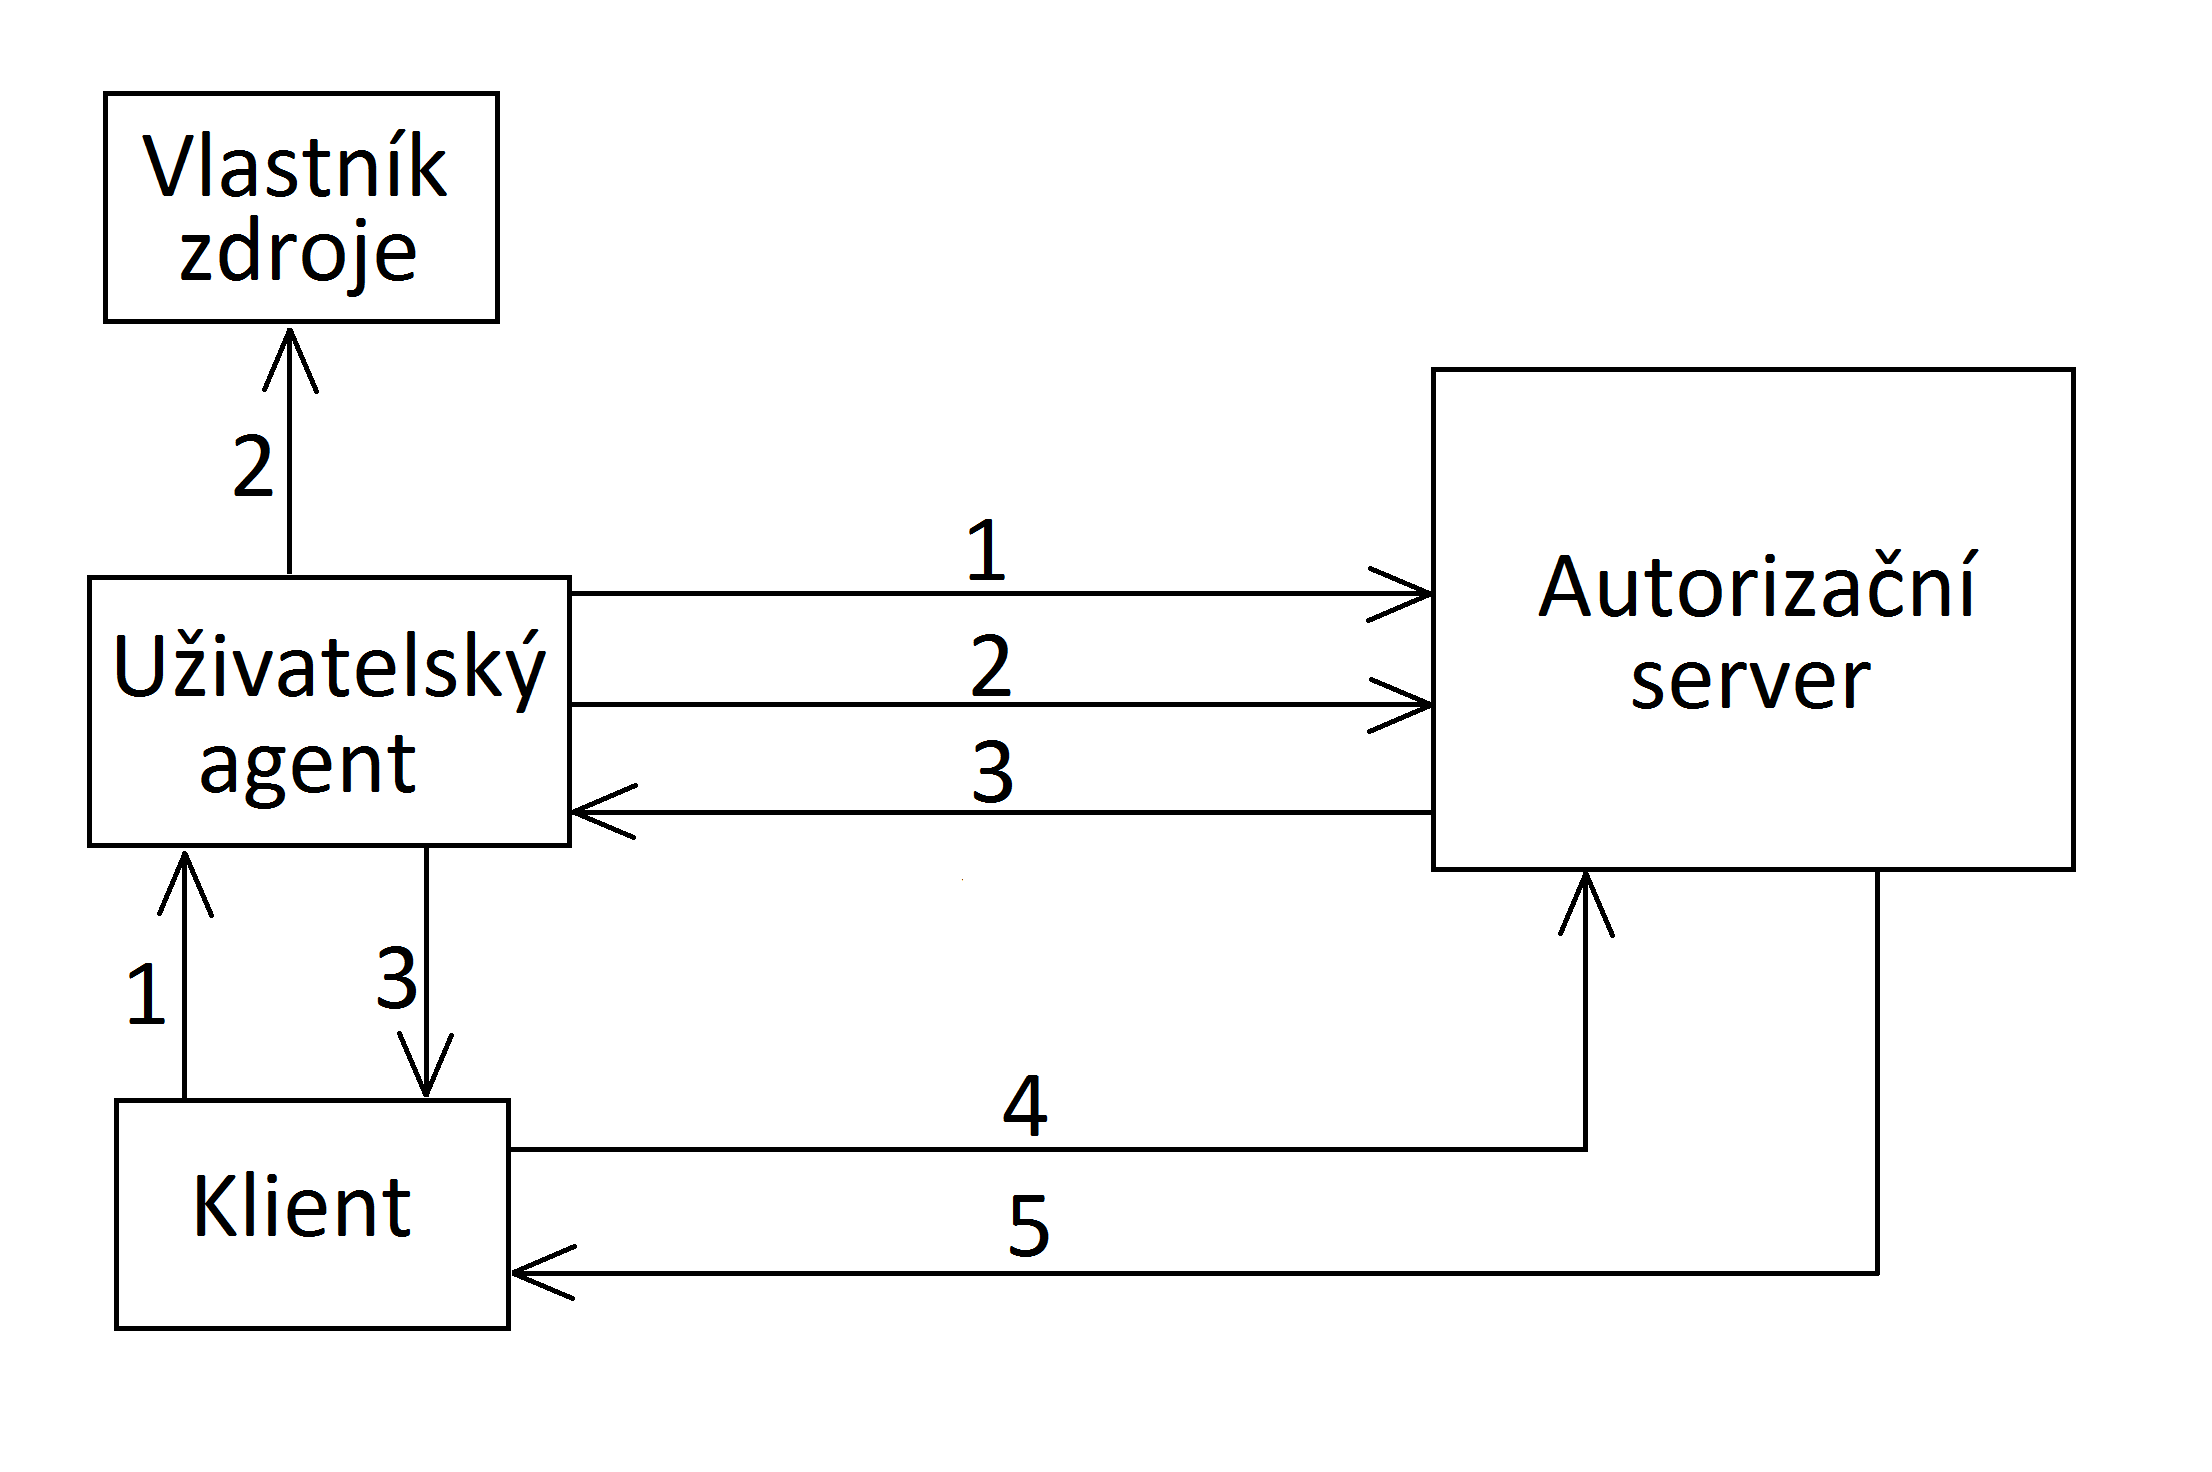
\includegraphics[width=\textwidth]{/home/oprikryl/Skola/bakalarka/oauth.png}
  		\end{minipage}
 		\caption{OAuth 2.0 - Autorizace autorizačním kódem.}
  		\label{fig:oauth}
	\end{figure}

	\begin{enumerate}
		\item {
		Klient pomocí prohlížeče přesměruje vlastníka zdroje na autorizační server. Klient v 				požadavku uvede svůj identifikátor, požadovaný rozsah přístupu,  identifikační řetězec
			\footnote {
			Identifikační řetězec (tzv. state) slouží k identifikaci sezení při větším počtu různých 				OAuth požadavků.
			}	 
		a adresu, na kterou má být zaslán autorizační kód.
		}
		\item
		Vlastník zdroje se autentizuje serveru a potvrdí klientovi přístup o daném rozsahu.
		\item
		Autorizační server přesměruje prohlížeč na adresu obdrženou v prvním kroku a předá ji 			autorizační kód a identifikační řetězec.
		\item
		Klient zažádá autorizační server o přístupový token. V požadavku uvede autorizační kód 			přijatý v předchozím kroku, identifikační údaje klienta a adresu použitou k získání 					autorizačního kódu v prním kroku. 
		\item	
		Autorizační server zkontroluje identifikační údaje klienta a ověří platnost autorizačního 				kódu. Jestliže jsou všechny údaje platné, autorizační server zašle přístupový token a 				obnobující token klientovi.

	\end{enumerate}


\end{document}